\section{Photomultiplier Tubes in the XENON100 experiment}
\label{secPMT}

%\begin{floatingfigure}[l]{0.22\textwidth}
%\begin{figure}[!h]
%\centering
%\subfigure[]{
%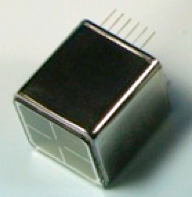
\includegraphics[height=0.2\linewidth]{plots/PMT/R8520.png}
%\label{figPMT_1}}
%\subfigure[]{
%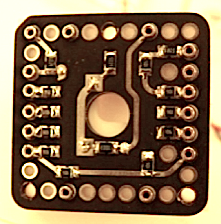
\includegraphics[height=0.2\linewidth]{plots/PMT/PMTbase.png}
%\label{figPMT_2}}
%\caption{R8520-06-AL Hamamatsu PMT (a) and the {\it Cirlex} base with the voltage divider network.}
%\label{figPMT}
%\end{figure}
%\end{floatingfigure}

XENON100 detector utilizes 242 1"-square Hamamatsu PMTs, shown in Fig.~\ref{figPMT_1}. Model R8520-06-AL has been specifically designed to operate in liquid xenon, and to withstand temperature in the range -110 to +50$^{\circ}$C and absolute pressure up to 5~atm. In collaboration with the company, the materials which are used to produce the PMTs have been screened with germanium spectrometers~\cite{ScreeningPaper}, and the design has been optimized to reduce the radioactive contamination.

% joined figure, all 3 pictures together
%\begin{floatingfigure}[l]{0.22\textwidth}
\begin{figure}[!h]
\centering
\subfigure[]{
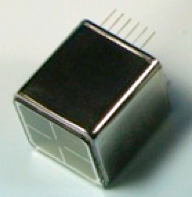
\includegraphics[height=0.20\linewidth]{plots/PMT/R8520.png}
\label{figPMT_1}}
\subfigure[]{
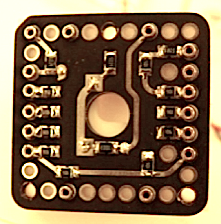
\includegraphics[height=0.20\linewidth]{plots/PMT/PMTbase.png}
\label{figPMT_2}}
\subfigure[]{
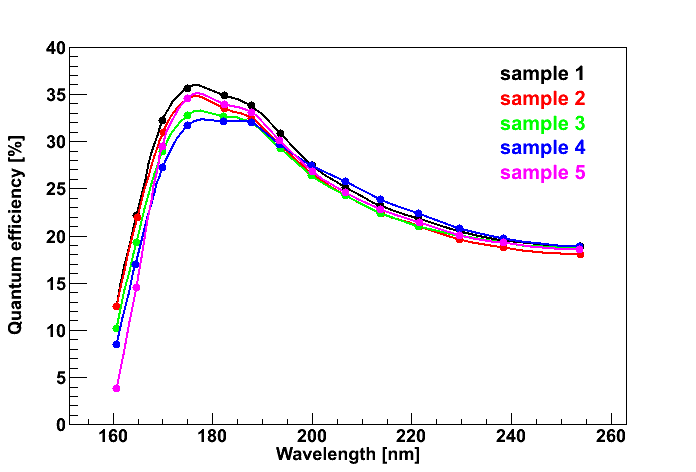
\includegraphics[width=0.475\linewidth]{plots/QE/plotQEvsWL_highQE.png}
\label{figPMT_3}}
\caption[R8520-06-AL Hamamatsu PMT with the voltage divider network on a {\it Cirlex} base, and its quantum efficiency as a function of the wavelength]{R8520-06-AL Hamamatsu PMT (a) with the voltage divider network on a {\it Cirlex} base (b), and quantum efficiency as a function of the wavelength (c)~\cite{PMTmassModel}.}
\label{figPMT}
\end{figure}
%\end{floatingfigure}

%\begin{figure}[!h]
%\centering
%\subfigure[]{
%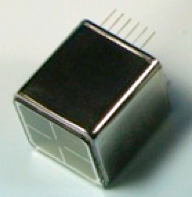
\includegraphics[height=0.2\linewidth]{plots/PMT/R8520.png}
%\label{figPMT_1}}
%\subfigure[]{
%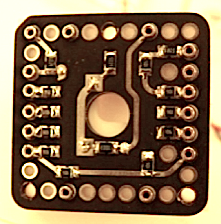
\includegraphics[height=0.2\linewidth]{plots/PMT/PMTbase.png}
%\label{figPMT_2}}
%\caption{R8520-06-Al Hamamatsu PMT (a) and the {\it Cirlex} base with the voltage divider network (b).}
%\label{figPMT}
%\end{figure}

The bialkali photocathode has a minimum effective area of 20.5$\times$20.5 mm, spectral response on the region 160-650~nm and the highest quantum efficiency (QE) for VUV light (see Fig.~\ref{figPMT_3}). The aluminum strips deposited on the window improve the resistivity of the photocathode at cryogenic temperature. The electron multiplier consists of 10 stage metal channel dynode structure. The PMT window is made out of synthetic silica, which has properties of quartz and transmits ultraviolet radiation down to 160~nm. The thermal expansion coefficient of silica is significantly different from that of {\it Kovar} alloy used for the stem pins. The bulb stem is thus made from borosilicate glass, and a graded seal using gradually different thermal expansion coefficient is connected to the synthetic silica bulb. 
The individual components of a R8520-06-AL Hamamatsu PMT are listed together with their total weight in Table~\ref{tabPMTmassModel}~\cite{PMTmassModel}.

Two types of R8520 PMTs are used in the XENON100 detector. The older type (`low QE' PMTs)  that has been also used in XENON10 has an average peak quantum efficiency of 25\%. The newer type of this model (`high QE' PMTs), with an improved photocathode, has a peak quantum efficiency of $\sim$32\% at 175~nm (Fig.~\ref{figPMT_3}).

%\begin{figure}[!h]
%\centering
%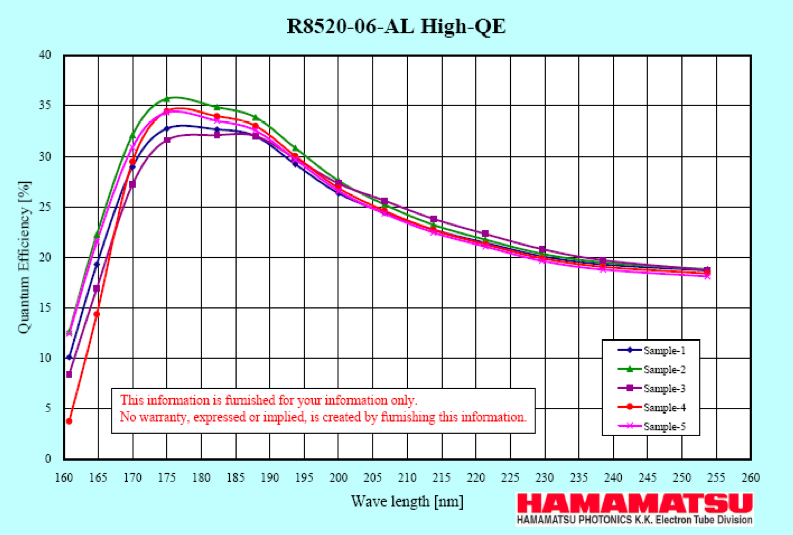
\includegraphics[width=0.475\linewidth]{plots/PMT/Hamamatsu_QEvsWavelength.png}
%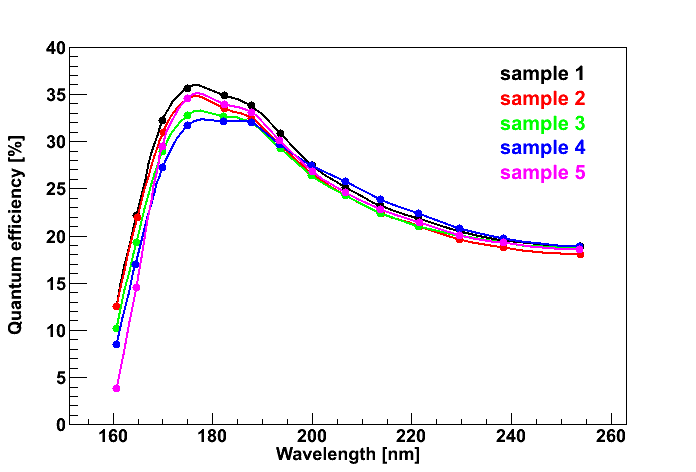
\includegraphics[width=0.475\linewidth]{plots/QE/plotQEvsWL_highQE.png}
%\caption[Quantum efficiency as a function of the wavelength for the 'high QE' Hamamatsu PMTs used in the XENON100 experiment]{Quantum efficiency as a function of the wavelength for the 'high QE' Hamamatsu PMTs used in the XENON100 experiment~\cite[PMTmassModel].}
%\label{figQEhighQE}
%\end{figure}

\begin{table}[!h]
\centering
\caption[Mass model of the R8520-06-AL PMT]{Mass model of the R8520-06-AL PMT \cite{PMTmassModel}.}
\label{tabPMTmassModel}
%\vspace{0.2cm}
\begin{tabular}{>{\footnotesize}l|>{\footnotesize}l|>{\footnotesize}c}
%\begin{tabular}{l|l|c}
\hline
PMT part 					& Material				& Weight [g] \\
\hline
Metal package and stem pins	& {\it Kovar} alloy 		& 13.0	\\
Electrodes				& stainless steel 		& 7.0 \\
Glass for window			& synthetic silica		& 2.0 \\
Glass in stem				& borosilicate glass		& 1.0 \\
Aluminum ring				& Al 					& 0.1	 \\
Insulator					& ceramic				& 0.04 \\
Getter					& ZrAl				& 0.02 \\
\hline
\end{tabular}
\end{table}

A PMT is supplied with high voltage via {\it Kapton} insulated wires. The voltage divider network, which is used to distribute the high voltage supplied to a PMT and provide a proper voltage gradient to each dynode, is shown in Fig.~\ref{figPMT_2}. It consists of 13 surface mount resistors and a capacitor, soldered on a substrate (base) made out of {\it Cirlex}~\cite{cirlex}. The cables used for the PMT signal are RG174 model, consisting of the copper conductor in PTFE isolation with a tinned copper shield~\cite{RG174cable}. The estimated total length of the cables in the detector is 530~m, with corresponds to a weight of 1.8~kg. 

The top array on the target volume consists of 98 PMTs, mounted in a concentric pattern inside the diving bell. The PMTs are installed in the PTFE disk-like structure (Fig.~\ref{figTopArray_1}) and are held on the top with oxygen-free high thermal conductivity (OFHC) copper rings (Fig.~\ref{figTopArray_2}).


\begin{figure}[!h]
\centering
\subfigure[]{
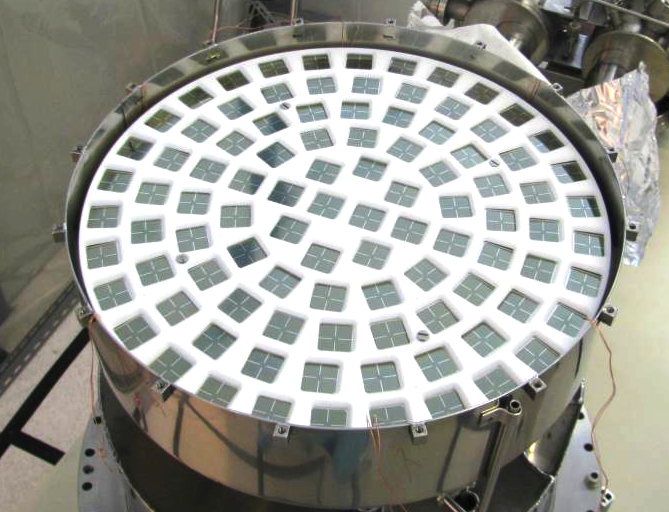
\includegraphics[height=0.3\linewidth]{plots/PMT/TopPMTarray_front.png}
\label{figTopArray_1}}
\subfigure[]{
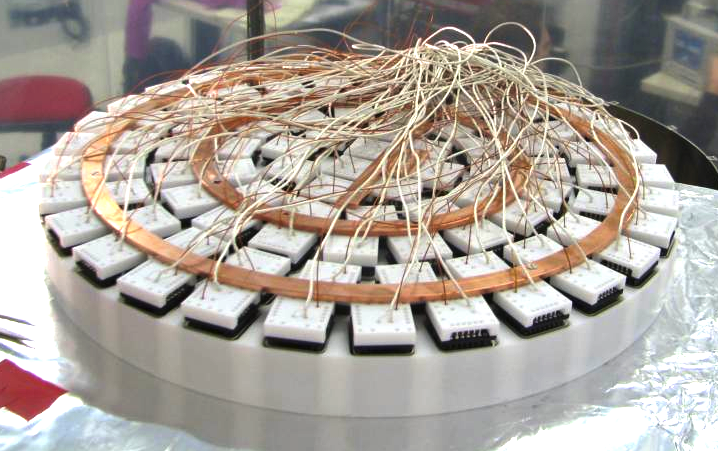
\includegraphics[height=0.3\linewidth]{plots/PMT/TopPMTarray_rear.png}
\label{figTopArray_2}}
\caption[Front and rear views of the top PMT array]{Front (a) and rear (b) views of the top PMT array, installed inside the diving bell in a PTFE structure with a copper support.}
\label{figTopArray}
\end{figure}

\begin{figure}[!h]
\centering
\subfigure[]{
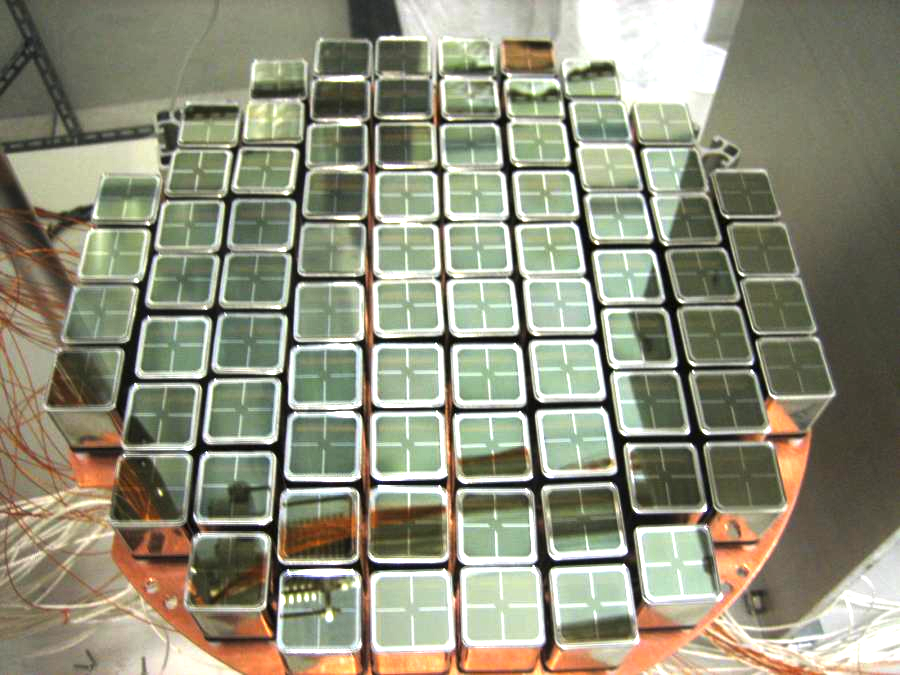
\includegraphics[height=0.3\linewidth]{plots/PMT/BottomPMTarray_front.png}
\label{figBottomArray_1}}
\subfigure[]{
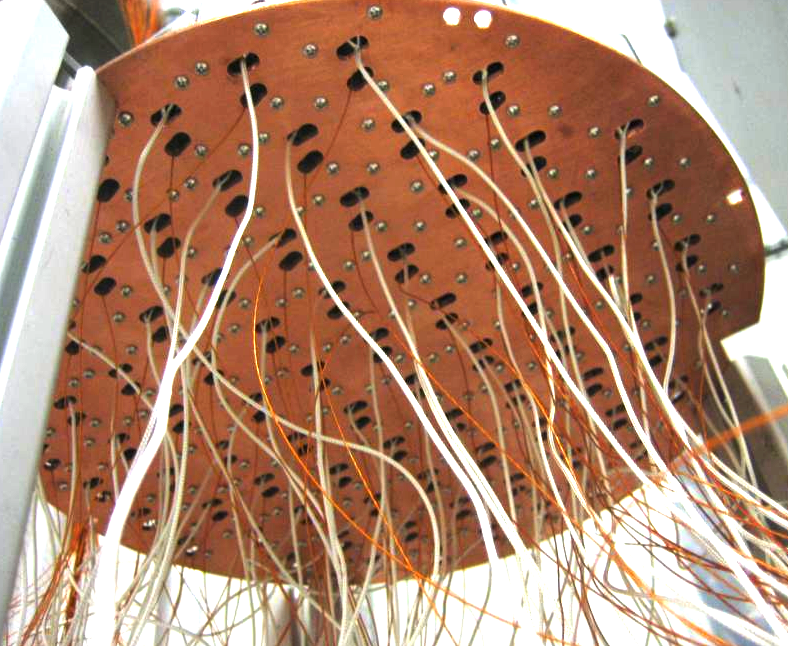
\includegraphics[height=0.3\linewidth]{plots/PMT/BottomPMTarray_rear.png}
\label{figBottomArray_2}}
\caption[Bottom PMT array in the target volume]{Bottom PMT array in the target volume (a), mounted on a copper plate (b).}
\label{figBottomArray}
\end{figure}

The bottom PMT array consists of 80 PMTs, mounted in a rectangular pattern in order to maximize the photocathode coverage (Fig.~\ref{figBottomArray_1}). They are mounted on a OFHC copper plate (Fig.~\ref{figBottomArray_2}).

The veto volume is equipped with 64 PMTs mounted on the copper angles and alternating the direction (Fig.~\ref{figVetoArrays}). 32 of them observe the sides from the top and bottom, and 32 PMTs view the veto volume above and below the TPC.

\begin{figure}[!h]
\centering
\subfigure[]{
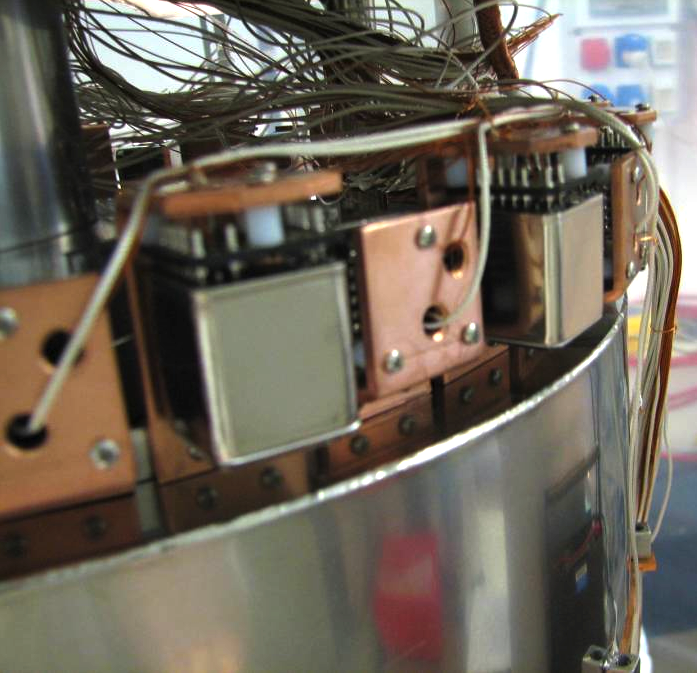
\includegraphics[height=0.3\linewidth]{plots/PMT/VetoTopPMTarray.png}
\label{figVetoArrays_1}}
\subfigure[]{
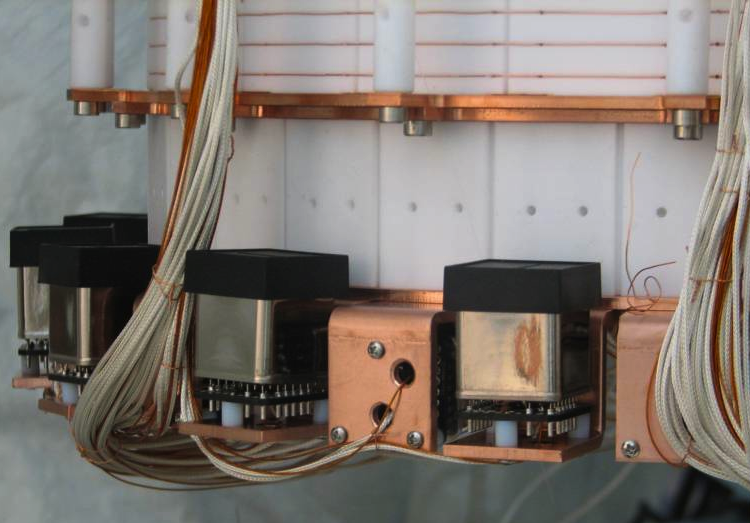
\includegraphics[height=0.3\linewidth]{plots/PMT/VetoBottomPMTarray.png}
\label{figVetoArrays_2}}
\caption[PMT arrays in the veto volume]{PMT arrays in the veto volume: (a) - top and upper side; (b) - bottom and lower side.}
\label{figVetoArrays}
\end{figure}

The arrangement of the PMTs within the target volume and veto arrays is shown in Fig.~\ref{figPMTarrangement}. 
At the beginning of the commissioning run in Fall~2009, 8 PMTs stopped working, mostly due to a connection problem or a shortcut inside the cryostat. For some of the PMTs, an increase of the dark current rate has been observed shortly before the failure, which might indicate a progressive deterioration of the vacuum sealing.

\begin{figure}[!h]
\centering
\subfigure[top]{
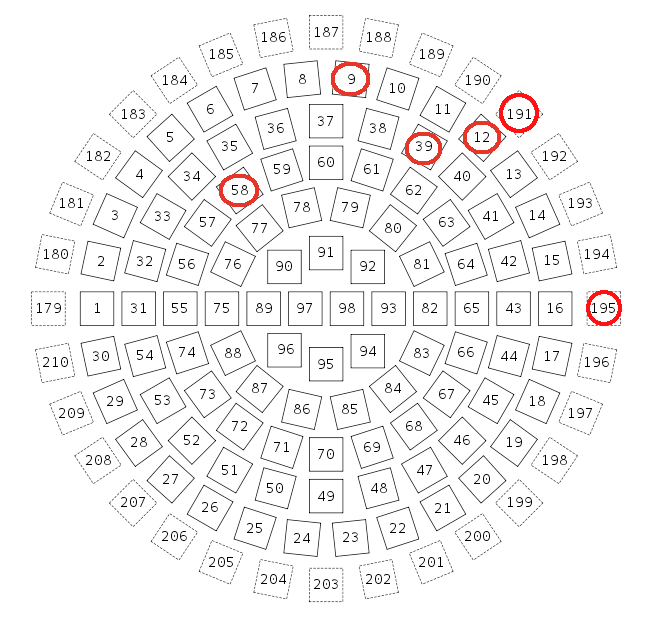
\includegraphics[height=0.425\linewidth]{plots/PMT/topPMTs.png}
\label{figPMTarrangement_1}}
\subfigure[bottom]{
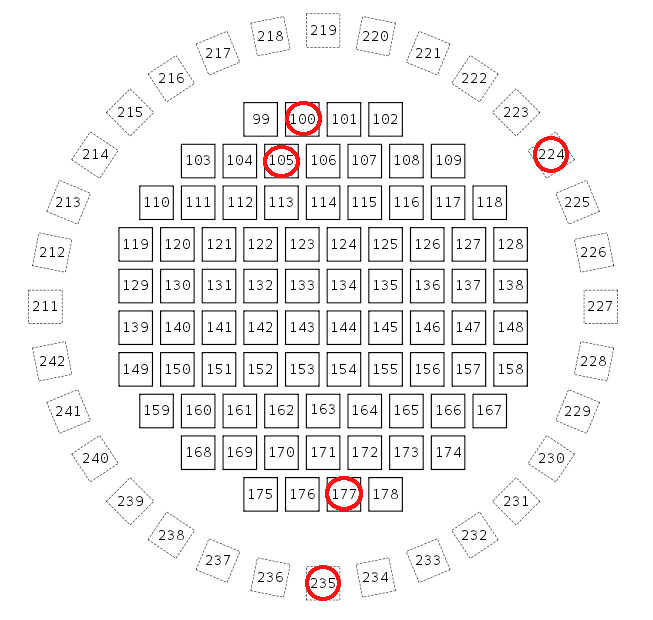
\includegraphics[height=0.425\linewidth]{plots/PMT/bottomPMTs.png}
\label{figPMTarrangement_2}}
\caption[The arrangement of the PMTs within the detector arrays]{The arrangement of the PMTs within the detector arrays. PMTs 1-98 - top array in the target, 99-178 - bottom array in the target, 179-210 - top and upper side arrays in the veto, 211-242 - bottom and lower side arrays in the veto. The red circles show the channels that are not functioning.}
\label{figPMTarrangement}
\end{figure}


